\paragraph{Scenarios}
    \begin{enumerate}
        \item Johnny is a model citizen of Milan and he is really caring about parking violations, because they are really frequent in his neighbourhood. When he see a violation, he opens the SafeStreets app on his smartphone and reports it with just few clicks. All he needs to do is to take a photo of the violation where the license plate is clearly visible and confirm if the system detected it correctly or not, if not he inserts the license plate manually in the field that appears after the confirmation. Position is automatically detected from the GPS because he allowed the app to access it, and to send the report to SafeStreets he just needs to confirm by clicking the done button.
        
        \item Giuseppe is a veteran user of SafeStreets app, registered to the system since its beginning. One day he need to update his e-mail, because he has no more access to the one he registered with, so he opens the app and check his account tab. Here, he clicks on update e-mail and inserts the new one, then he logs in the e-mail service to confirm the change.
    \end{enumerate}

\begin{figure}[H]
	\centering
    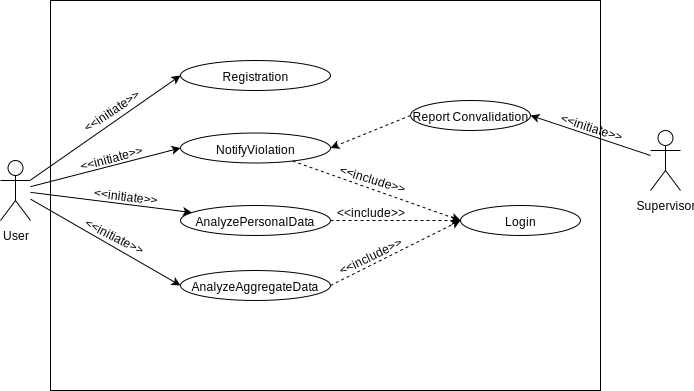
\includegraphics[width=\textwidth]{UML/UseCaseUser}
\end{figure}	

\textbf{Use cases}\\

\begin{tabular}{|p{3.1cm}|p{11.6cm}|}
\hline
Name & Registration\\
\hline
Actors & Citizen\\
\hline
Entry Condition & The user opens the app and has no valid account.\\
\hline
Event flow & \begin{enumerate}
                \item The user inserts the desired username.
                \item The user inserts the desired password.
                \item The user confirms his password.
                \item The user inserts his email.
                \item The user inserts his birthday.
                \item The user agrees to the use of his personal data and of his submitted violation reports for analysis purposes.
            \end{enumerate}\\
\hline
Exit condition & The registration is successful and the user is redirected to login form.\\
\hline
Exception & Email is already in use or confirm password field content diverge from password, in this case the user is alerted with a proper message on screen and asked to correct the data.\\
\hline
\end{tabular}

\vskip 0.2in
\begin{tabular}{|p{3.1cm}|p{11.6cm}|}
\hline
Name & Login\\
\hline
Actors & Citizen\\
\hline
Entry Condition & The citizen opens the app.\\
\hline
Event flow & \begin{enumerate}
                \item The citizen inserts his email.
                \item The citizen inserts his password.
                \item The citizen press the login button.
            \end{enumerate}\\
\hline
Exit condition & The citizen is authenticated and login is successful.\\
\hline
Exception & Username or password are invalid, "invalid credentials" message is displayed and the citizen needs to insert credentials again.\\
\hline
\end{tabular}

\vskip 0.2in
\begin{tabular}{|p{3.1cm}|p{11.6cm}|}
\hline
Name & Notify violations\\
\hline
Actors & Citizen\\
\hline
Entry Condition & Violation detection.\\
\hline
Event flow & \begin{enumerate}
                \item The User selects the report tab if not already selected.
                \item The User selects the type of violation.
                \item The User takes and uploads a photo of the violation.
                \item The User confirms that the license plate is correctly recognized by app, if not he/she inserts it manually in the appropriate field.
                \item The User checks whether his/her current position is correctly identified by the GPS system, if not he/she inserts it manually in the appropriate field.
                \item The User confirms the violation report clicking on the "Done" button.
                \item The system stores the information and completes it with suitable metadata.
                \item The system sends a notification to the User about the success of the operation.
            \end{enumerate}\\
\hline
Exit condition & The violation report is correctly stored.\\
\hline
Exception & the system detects missing information and rejects the report, then asks the User for missing data.\\
\hline
\end{tabular}

\vskip 0.2in
\begin{tabular}{|p{3.1cm}|p{11.6cm}|}
\hline
Name & Analyze aggregate data\\
\hline
Actors & Citizen\\
\hline
Entry Condition & The citizen wants to know some information about the reported violations.\\
\hline
Event flow & \begin{enumerate}
                \item The citizen selects the "aggregated data" tab.
                \item The citizen selects the topic he/she is interested about.
                \item The citizen may select an appropriate filter for his search.
                \item The citizen selects the data of interest.
                \item The system provides the data to be visualized according to the actor's authorization level.
                \item The citizen visualizes the data.
            \end{enumerate}\\
\hline
Exit condition & The Actor finishes to analyze the data.\\
\hline
\end{tabular}

\vskip 0.2in
\begin{tabular}{|p{3.1cm}|p{11.6cm}|}
	\hline
	Name & Check personal reports\\
	\hline
	Actors & Citizen\\
	\hline
	Entry Condition & The citizen opens the app, desiring to check the reports he sent in the past.\\
	\hline
	Event flow & \begin{enumerate}
		\item The citizen selects the account tab.
		\item The citizen clicks on "View reports sent" button.
		\item The system displays a list of all reports done by the citizen.
		\item The citizen clicks on a report to see his details.
		\item The citizen clicks the return button, going back to the list of reports.
		\item The citizen can repeat the last two steps as many times as he pleases, to check other reports.
	\end{enumerate}\\
	\hline
	Exit condition & The citizen closes the reports list after he doesn't need to visualize them anymore.\\
	\hline
\end{tabular}

\vskip 0.2in
\begin{tabular}{|p{3.1cm}|p{11.6cm}|}
	\hline
	Name & Update e-mail\\
	\hline
	Actors & Citizen\\
	\hline
	Entry Condition & The citizen opens the app, desiring to change the e-mail associated to his account.\\
	\hline
	Event flow & \begin{enumerate}
		\item The citizen selects the account tab.
		\item The citizen clicks on "Change e-mail" button.
		\item The citizen inputs a new e-mail in the pop-up.
		\item The citizen checks the input of the given e-mail, opens the e-mail concerning his e-mail change and clicks on a link to confirm the change.
		\item A confirmation about the success of the operation is printed on screen after the link is opened.
	\end{enumerate}\\
	\hline
	Exit condition & The confirmation message correctly appears on user's device screen.\\
	\hline
	Exception & Email is already in use or it has an invalid format, the user is then asked to input another e-mail in the field. If the e-mail for confirming the change of the account's e-mail is not correctly received by the user for any reason, he/she can contact the support about the issue.\\
	\hline
\end{tabular}

% sequence diagrams
\newpage
\textbf{Sequence diagrams}
\begin{figure}[H]
	\centering
	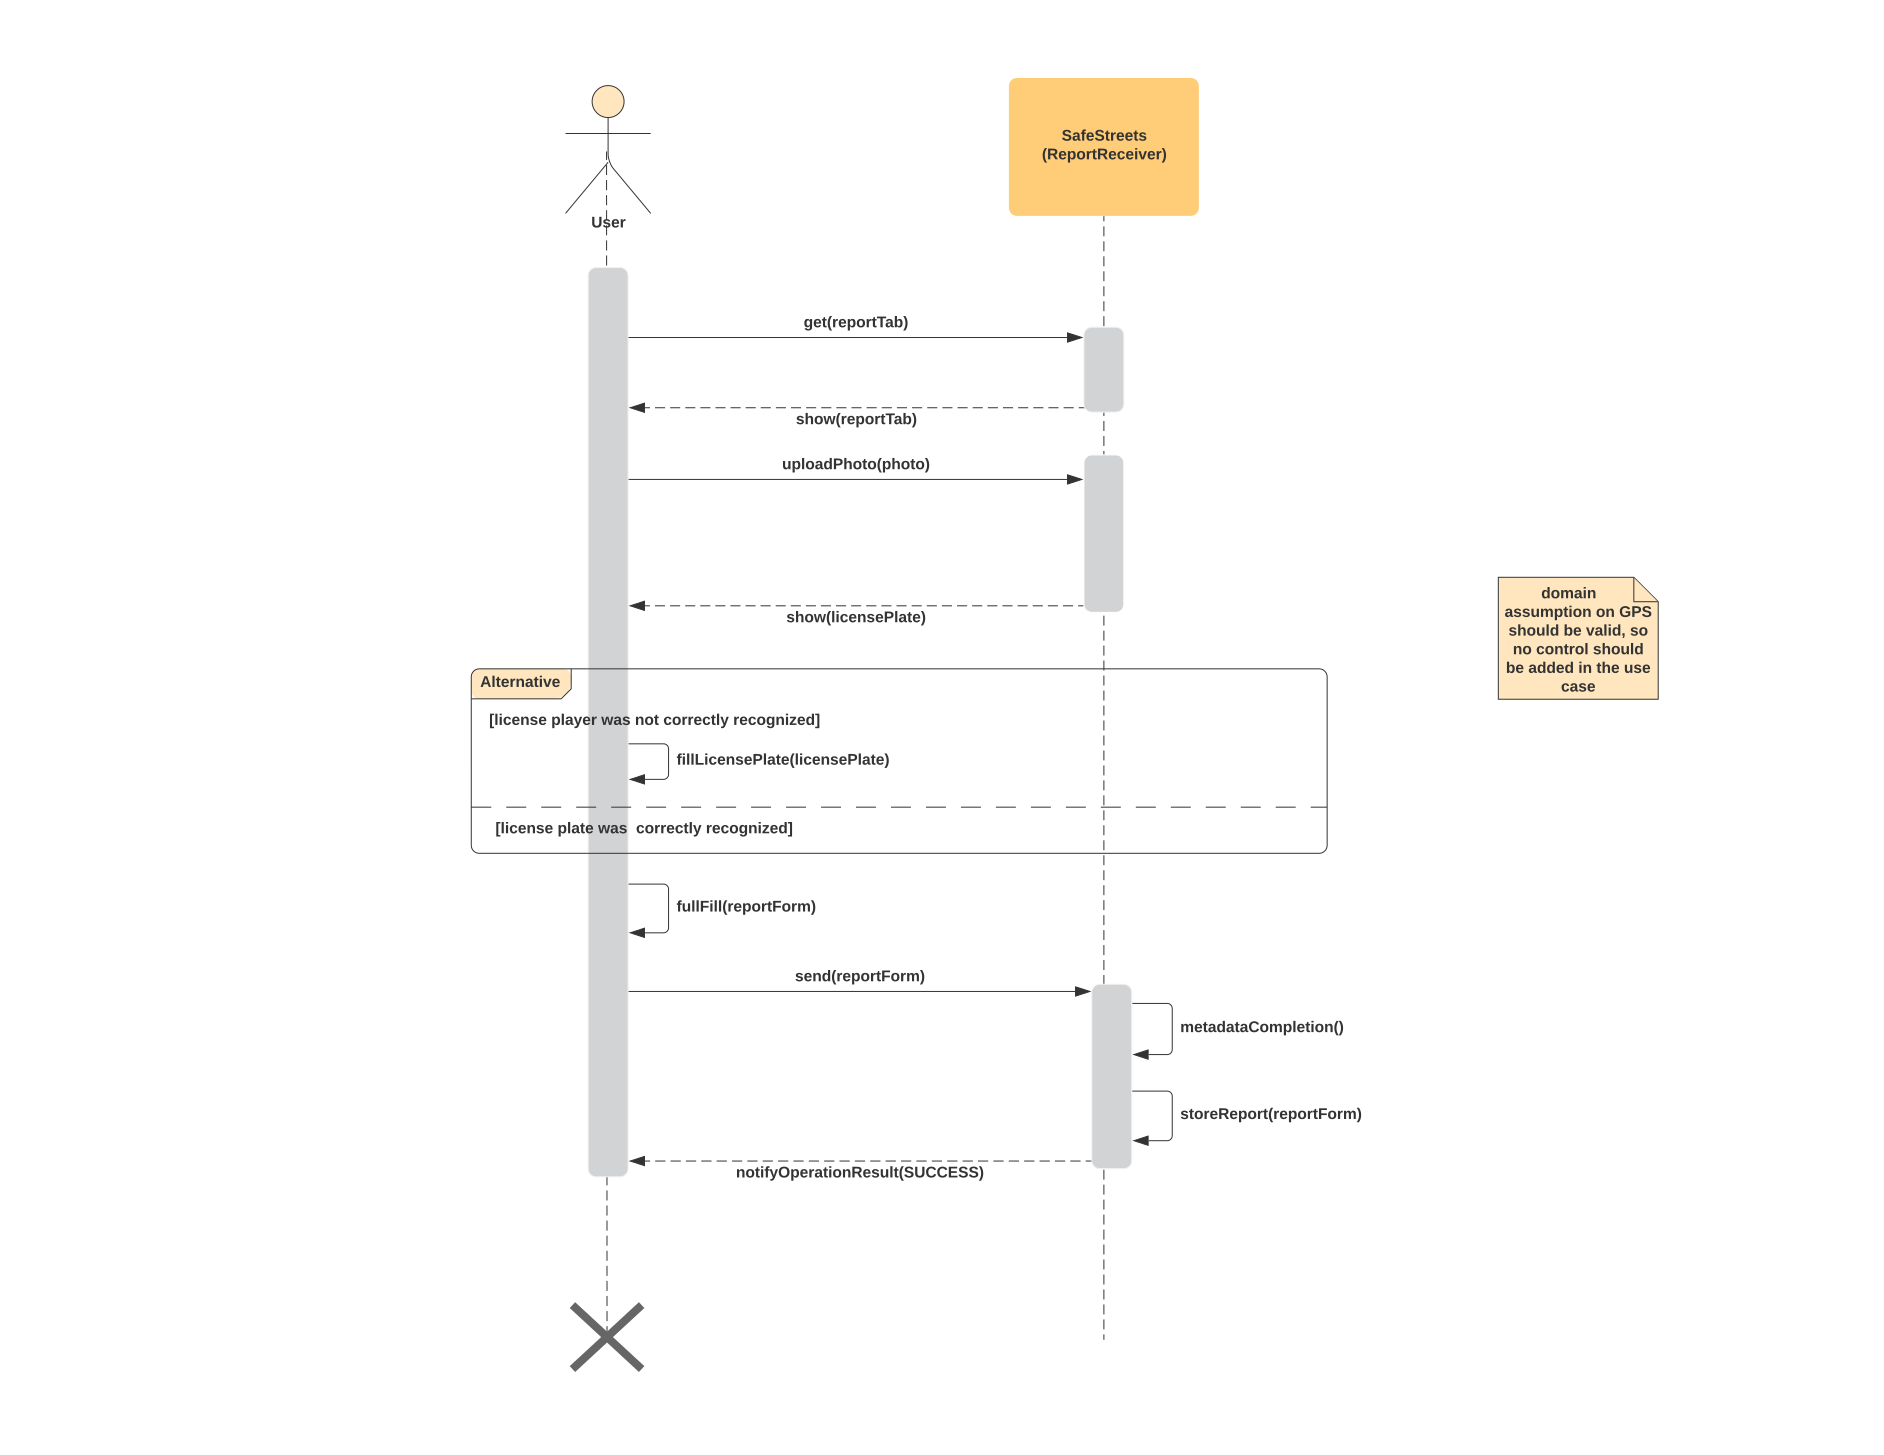
\includegraphics[width=\linewidth]{Images/UML/NotifyViolationUseCase}
	\caption{Notify violation use case.}
\end{figure}
\begin{figure}[H]
	\centering
	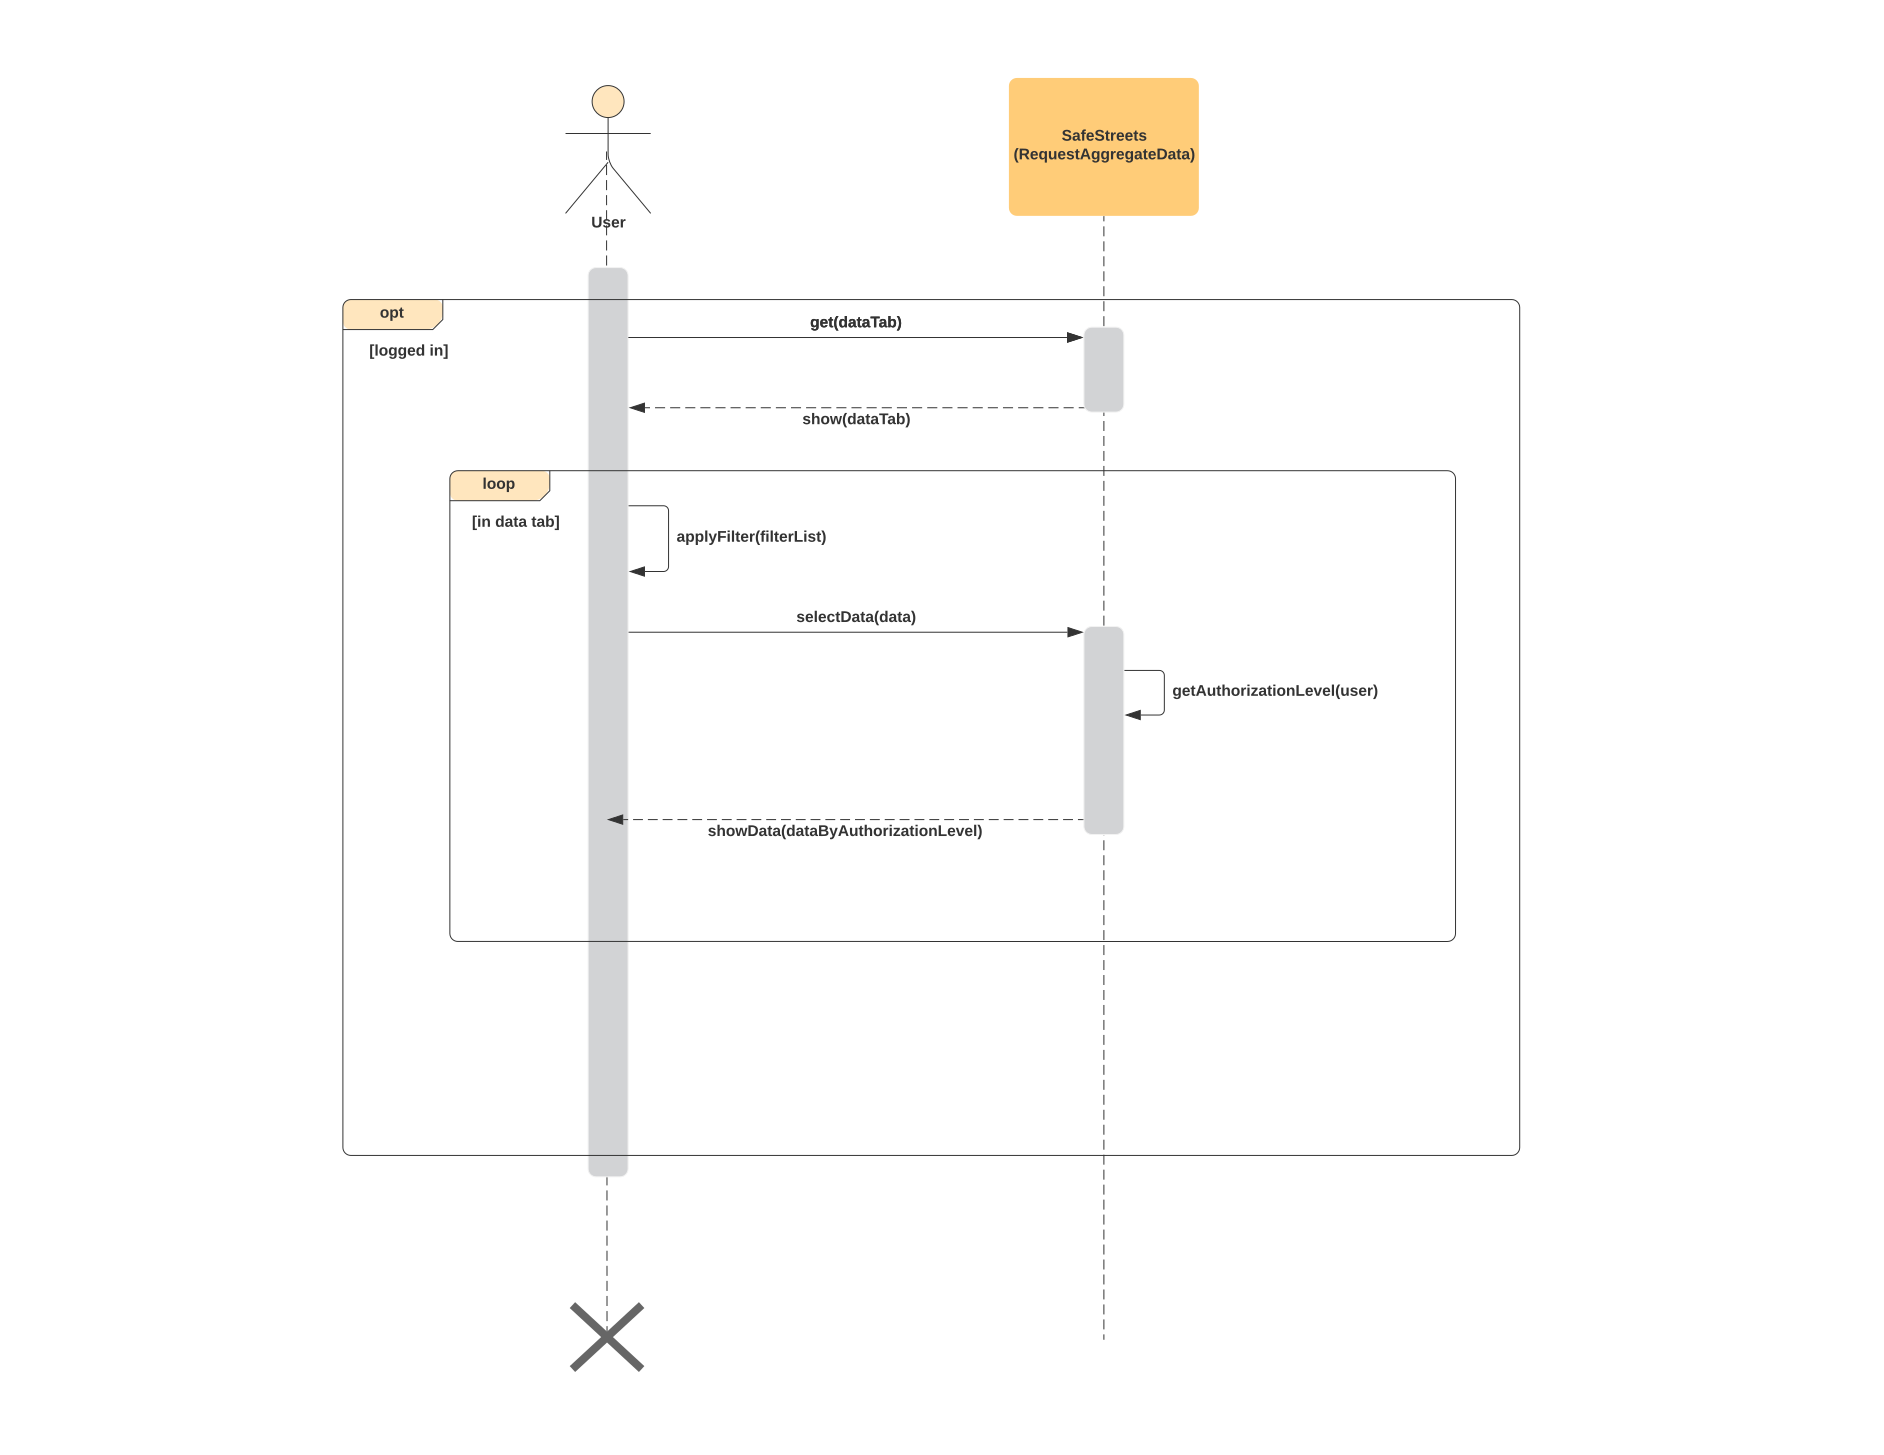
\includegraphics[width=\linewidth]{Images/UML/AnalyzeDataUseCase}
	\caption{Analyze aggregate data use case.}
\end{figure}
